\documentclass[11pt,oneside,a4paper]{article}     % onecolumn (second format)
\usepackage[T1]{fontenc}
\usepackage[english]{babel}
\usepackage[utf8]{inputenc}
\usepackage{epstopdf}
% GRAPHICS AND IMAGES

\usepackage{mathtools}
\usepackage{acronym}
\usepackage{graphicx}
\usepackage{amsthm}
\usepackage{amsmath}
\usepackage{amssymb}
\usepackage{tabularx}
\usepackage[algoruled, vlined, linesnumbered]{algorithm2e}% http://ctan.org/pkg/algorithms
%\usepackage{algpseudocode}
% INCLUDE YOUR PACKAGES HERE
%\usepackage{amsfonts,amsmath,amsthm, amssymb}
\usepackage{subfig}
\usepackage[font=scriptsize]{caption}
\usepackage[dvipsnames]{xcolor}
\newcommand*{\dt}[1]{\accentset{\mbox{\large\bfseries .}}{#1}}

\newcommand{\ind}{1{\hskip -2.5 pt} \mathrm{I}}


\newtheorem{definition}{Definition}
\newtheorem{lemma}{Lemma}
\newtheorem{prop}{Proposition}
\newtheorem{assumption}{Assumption}
\newtheorem{theorem}{Theorem}
\newtheorem{remark}{Remark}
\newtheorem{corollary}{Corollary}

\newenvironment{sistema}%
{\left\lbrace\begin{array}{@{}l@{}}}%
{\end{array}\right.}

\DeclareMathOperator*{\argmax}{arg\,max}
\DeclareMathOperator*{\argmin}{arg\,min}
\DeclareMathOperator*{\lexmax}{lex\,max}

\title{Iterative LexMax fair tutor-student assignment}

\date{\today}
\author{MegaMath4SmallBiz, Frateli}


\begin{document}
\maketitle


\section{Scenario}

Let $S,T$ be the set of students and tutors, respectively. For each student/tutor pair $(s,t)$ there exists a score $a_{s,t}$ that measures the affinity between student $s$ and tutor $t$.

Each tutor $t$ can mentor at most $N_t$ students. On the contrary, there is no bound on the number of tutors that can mentor the same student. More formally, let $x_{s,t}=\{0,1\}$ be the binary variable that equals 1 if and only if tutor $t$ is assigned to student $s$. Then, 
\begin{equation} \label{eq:constr1}
\sum_{s\in S} x_{s,t} \le N_t, \qquad \forall\, t\in T.
\end{equation}



\subsection{Related works}

If each tutor can only mentor exactly one student ($N_t=1$ for all $t\in T$) then our problem is similar to the one studied in \cite{santaclaus06} and  \cite{chakrabarty2009allocating}. 



\section{Desiderata}

We wish to find a tutor-student assignment $x^*$ with the following desiderata:
\begin{enumerate}
\item $x^*$ must respect constraint (\ref{eq:constr1}), i.e., each tutor $t$ cannot supervise more than $N_t$ students;
\item $x^*$ must take into account that student preferences are not linear in the affinities $r$ with the assigned tutors. For instance, a student $s$ arguably prefers to be assigned to a single tutor $t$ with affinity $10$ ($a_{s,t}=10$) rather than to two tutors with affinity equal to 5 each;
\item $x^*$ must be somehow ``fair'', thus it should intuitively avoid stark disparity among students. For instance, attempting to maximize the sum of affinities over all students and tutors is in general a bad idea since it does not guarantee fairness.
\end{enumerate}



\section{Preliminaries: max-min fairness}

We first observe that attempting at maximizing the total reward (call it \emph{max-sum}) over all students, measured as the sum of affinities with the assigned tutors, is in general not a good idea since it generates stark inequalities among students. In fact, the solution in this case is to let each tutor $t$ choose the $N_t$ students with the highest affinity. In other words, each tutor $t$ ranks the students in order of decreasing affinity $a_{s_1,t}\ge a_{s_2,t} \ge \dots$ and selects the first $N_t$ of them. However, there may be students with very low reward; potentially, there may be students $s$ with no tutors is assigned to them.

\begin{figure}[h!]
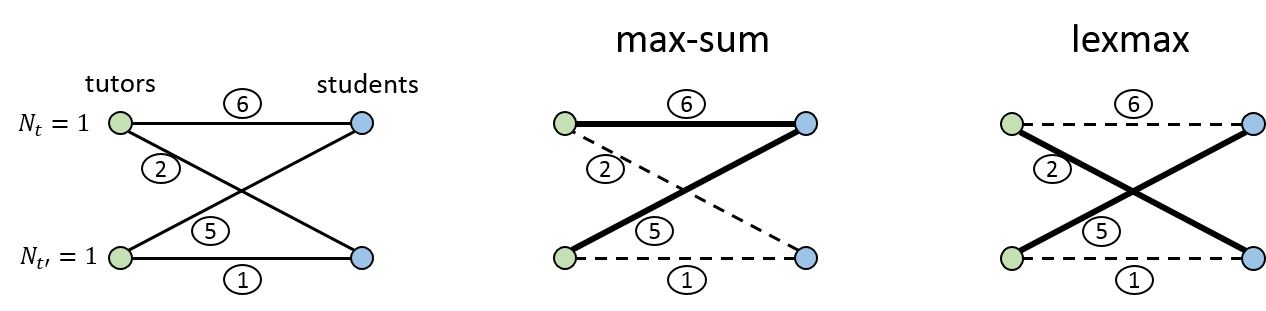
\includegraphics[scale=.6]{figs/example.png}
\caption{Comparison between max-sum and lexmax allocation. Max-sum maximizes the sum of affinities over all student-tutor pairs ($=11$ here) while lexmax finds iteratively the max-min allocation.}
\label{fig:example}
\end{figure}


For the reason outlined above, we aim at finding a ``fair'' assignment between students and tutors. To this aim, let us first define the crucial concept of max-min fairness.

\begin{definition}[Lexicographic ordering]
Let $A\in \mathbb{R}^n$ be a real vector. Let $\overline{A}$ denote $A$ sorted in increasing order. We say that $A\succ A'$ if $\overline{A}$ is lexicographically greater than $\overline{A}'$, i.e., $\exists \, n$ such that $\overline{A}_i=\overline{A}'_i$ for $i=1,\dots,n$ and $\overline{A}_{n+1}>\overline{A}'_{n+1}$. If $A\succ A'$ or $A=A'$ we write $A \succeq A'$.
\end{definition}

\begin{definition}[Max-min fair allocation] \cite{nace2008max}
% An allocation $a^*$ is max-min fair when the only way to increase the reward $a_s^*$ of a student $s$ is by decreasing the reward of a students $s'$ with lower reward, i.e., such that $x^*_{s'}< x^*_{s'}$.
Let $\mathcal F$ be the set of feasible allocations. 
The max-min fair allocation $A^*$ is the lexicographic maximum among all allocations in $\mathcal F$, and we write $A^*=\lexmax_{A\in \mathcal F} A$. In other words,
\[
A^*\succeq A, \quad \forall\, A\in \mathcal F.
\]
\end{definition}

Max-min fairness always give priority to students with smaller affinity with tutors (that would end up with a poor reward if we simply maximized the sum of rewards), and try to maximize their reward in an iterative fashion. For a good survey on max-min fairness we refer to \cite{nace2008max}.

Before showing how to apply the lexmax concept to our problem, let us show first a general-purpose algorithm to compute\footnote{We remark that this should still be regarded as a heuristic. In order to compute the exact lexmax, one should also find among all solutions to the \texttt{REFINE} step the one that ensures that lexmax is preserved in the subsequent steps. However, this would complicate further the algorithm, hence for the time being we will consider this version.} the lexmax allocation.

\begin{algorithm}[H]
\KwData{Feasible set $\mathcal F$}
\KwResult{Max-min fair allocation $a^*$}
\While{$|S|>0$}{
\textcolor{red}{\texttt{MAX-MIN:}} Compute $y = \max_{A\in \mathcal F} \, \min_{k\in S} \, A_k$.\\
\textcolor{red}{\texttt{REFINE:}} Find the allocation $A^*$ with minimum number of elements equal to $y$. Let $U=\{s:A^*_s=y\}$. \label{line1}\\
Set $A^*_{s}=y$ for all $s\in U$.\\
\textcolor{red}{\texttt{UPDATE:}} Update $\mathcal F:= \{A \in \mathcal F: \, A_{s}=y, \ \forall\, s \in U\}$.\\
Update $S := S\setminus U$.
}
\caption{General-purpose \textcolor{red}{\texttt{LEXMAX}} algorithm}
\label{alg:lexmax-genpurp}
\end{algorithm}





\section{Iterative LexMax assignment}

We now describe our approach to fairly assign tutors to students, according to the concept of max-min fairness described in the previous section.

The most natural idea would be to apply the concept of max-min fairness to the vector $A(x)$, whose element $s$ measures the sum of affinities student $s$ and the assigned tutors, i.e., $A_s(x)=\sum_{t}x_{s,t}\, a_{s,t}$. In other words, one would solve:
\[
\lexmax_{x\in \mathcal F} A(x)
\]
where $\mathcal F$ is the feasibility set $\{x\in\{0,1\}:\sum_{s\in S} x_{s,t}\le N_t, \ \forall\, t\in T\}$.
On the other hand, this would lead to a solution that does not well adapt to desiderata 2, since the linearity of $A(x)$ does not incorporate the fact that students prefer to be assigned with few tutors with high affinity rather than several tutors with low affinity.

Therefore, we propose an iterative algorithm that assigns at most \emph{one} tutor to each student at each iteration in a lexmax fashion, as long as the constraints on the maximum number of students supervised by the tutors are fulfilled. Namely, at each iteration a problem of this kind has to be solved:
\begin{align*}
& \, \lexmax_{x\in \mathcal F} A(x) \\
\mathrm{s.t.} & \, \sum_{t\in T} x_{s,t}\le 1, \quad \forall\, s\in S.
\end{align*}


We remark that by assigning only one tutor at the time, we tend to ensure high individual affinity for all students for the very first few iterations, which is in line with desiderata 2. 

\noindent The formal description of our procedure can be found in Algorithm \ref{alg:lexmax} below.

\begin{algorithm}[H]
 \KwData{Students $S$, tutors $T$, student-tutor affinity $a_{s,t}$, set of tutors $T_s=\{t:a_{s,t}>0\}$ available to student $s$}
 \KwResult{Max-min fair student-tutor assignment $\tau$. ($\tau_k(s)\subset T$ is the set of tutors assigned to student $s$ at iteration $k$)}
\textbf{Initialization}: Set $S'':=\emptyset$ (unassigned students) and $k:=0$. \newline
\textbf{Procedure}:\\
\While{$(\exists \, t: \, N_t>0) \land (\exists \, s: \, |T_s|>0)$}{
Set $S':=S\setminus S''$.\\
Increment iteration count $k:=k+1$.\newline
\textcolor{red}{\texttt{LEXMAX}:} \emph{Allocate \emph{one} tutor to each student in lexmax fashion}: \\
\While{$(S'\ne \emptyset) \land (\exists \, t: \, N_t>0)$}{
\textcolor{red}{\texttt{MAX-MIN}:} Solve the max-min problem (MM) via Alg. \ref{alg:dichot}:
\begin{equation} \label{eq:maxmin1}
\begin{sistema}
\widetilde{y}_k = \max_x y  \\
\mathrm{s.t.} \, \sum_{t\in T_s} x_{s,t} \, a_{s,t} \ge y \qquad \forall\, s\in S' \\
\hspace{.67cm} \sum_{t\in T_s} x_{s,t} \le 1 \qquad \forall\, s\in S' \\
\hspace{.67cm} \sum_{s} x_{s,t} \le N_t \qquad \forall\, t\in T \\
\hspace{.67cm} x_{s,t} \in \{0,1\}, \quad \forall\, s,t.
\end{sistema} \tag{MM}
\end{equation}\\

\If{$\widetilde{y}_k=0$}{
Let $S^u$ be the set of unassigned students. Set $S':=S'\setminus S^u$ and $S'':=S''\cup S^u$. Decrement $k:=k-1$.
}
\Else{
\textcolor{red}{\texttt{REFINE:}} \emph{Find among all allocations solving \eqref{eq:maxmin1} the one with minimum number of pairs with affinity $=y_k$}:\newline
Let $E(y_k)\subset \mathcal{P}(y_k)$ be the set of student-tutor pairs with affinity equal to $y_k$, computed via \eqref{eq:maxmin1}. Then, solve the Min-Cost Flow problem (MCF):
\begin{equation}
\begin{sistema}
x^* = \argmin_x \, \sum_{(s,t)\in E(y_k)} x_{s,t}  \\
\mathrm{s.t.} \, \sum_{t:(s,t)\in \mathcal P(y_k)} x_{s,t}= 1, \qquad \forall \, s\in S' \\
\hspace{.67cm} \sum_{s:(s,t)\in \mathcal P(y_k)} x_{s,t} \le N_t, \qquad \forall\, t\in T \\
\hspace{.67cm} x_{s,t}\in \{0,1\}, \qquad \forall\, (s,t)\in \mathcal P(y_k).
\end{sistema} \tag{MCF}
\end{equation}
\label{line:hard}\\ 
\textcolor{red}{\texttt{UPDATE:}} Assign the tutors to the students accordingly: $\tau_k(t)= s$, $\forall\, (s,t):x^*_{s,t}=1$. \\
Update the set of students yet to be assigned to a tutor: $S':=S'\setminus \{s:\exists \,t: x^*_{s,t}=1\}$.\\
Update the number of available slots for each tutor $t$: $N_t:=N_t-\sum_s x^*_{s,t}$.\\
Update the set of available tutors for each student: $T_{s}:=T_{s}\setminus \{t:x^*_{s,t}=1\}$}
}}
\caption{Iterative LexMax fair tutor-student assignment}
\label{alg:lexmax}
\end{algorithm}



\subsection{Dichotomy search for Max-Min problem (MM)}

We now discuss how to solve the max-min problem \eqref{eq:maxmin1} at the generic iteration $k$, that asks to compute the maximum affinity $y_k$ such that all students are supervised by one tutor with affinity at least $y_k$. 

We perform a dichotomy search on all possible $M$ affinity values, considering only the student-tutor connections $\mathcal P(\alpha)$ with affinity not smaller to the current affinity value $\alpha$ and solving an appropriate Max-Flow problem MF($\alpha$), as discussed in Section \ref{sec:MF}. Then, each student can be supervised by a tutor with affinity $\ge \alpha$ if and only if the max-flow optimal value $f(\alpha)=|S'|$.\\



\begin{algorithm}[H]
 \KwResult{Max-min value $\widetilde y_k$ of \eqref{eq:maxmin1}.}
\textbf{Initialization}: Rank the scores $\{a_{s,t}\}_{s\in S',t\in T_s}$ in increasing order, eliminate the values appearing more than once and form the vector $\alpha_1,\alpha_2,\dots,\alpha_M$, where $M\le \sum_{s\in S'}|T_s|$. Set $l=1$ and $u=M$. Define $\mathcal P(\alpha)=\{(s,t), s\in S',t\in T_s: \, a_{s,t}\ge \alpha\}$. Then, denote by MF($\alpha$) the following Max-Flow problem:
\begin{equation} \label{eq:setcover2}
\begin{sistema}
f(\alpha) = \max_x \sum_{(s,t)\in \mathcal P(\alpha)} x_{s,t} \\
\sum_{t:(s,t)\in \mathcal P(\alpha)} x_{s,t} \le 1, \qquad \forall \, s\in S' \\
\sum_{s:(s,t)\in \mathcal P(\alpha)} x_{s,t} \le N_t, \qquad \forall\, t\in T \\
x_{s,t}\in \{0,1\}, \qquad \forall\, (s,t)\in \mathcal P(\alpha)
\end{sistema} \tag{MF($\alpha$)}
\end{equation}\newline
\textbf{Procedure}: \\
Solve MF($\alpha_l$) (see Section \ref{sec:MF}). Let $S^u=\{s:\sum_t x_{s,t}=0\}$ be the set of unassigned students\\
\If{$f(\alpha_l)<|S'|$}{
\textbf{Return} the max-min optimal value $\widetilde y_k:=0$ and $S^u$.}
Solve MF($\alpha_u$)\\
\If{$f(\alpha_u)=|S'|$}{
\textbf{Return} the max-min optimal value $\widetilde y_k:=\alpha_h$ and $S^u=\emptyset$.}
\While{$|u-l|>1$}{
Solve MF($\alpha_m$), where $m=\lceil \frac{l+u}{2}\rceil$
\\
\If{$f(\alpha_m)=|S'|$}{
Set $l:=m$
}
\Else{
Set $r:=m$
}}
\textbf{Return} the max-min optimal value $y_k:= \alpha_l$ and $S^u=\emptyset$.
\caption{Dichotomy search for Max-Min problem \eqref{eq:maxmin1}}
\label{alg:dichot}
\end{algorithm}


We remark that the dichotomy search needs $\mathcal O(\log_2 M)$ iterations, therefore the Iterative Max-min Algorithm \ref{alg:lexmax} has complexity $\mathcal O(M\log_2 M)$, where $M$ is the number of different affinity values.

One possibility to reduce the algorithm complexity is is to aggregate the affinity values to lower $M$.

\subsection{Max-Flow (MF)} \label{sec:MF}


We now explain how the problem (MF) can be recast as a classic max-flow one, that answers in \emph{polynomial time} to the following question: ``\emph{Given a capacitated graph and two nodes $v,v'$, what is the maximum amount of flow that can be carried from $v$ to $v'$?}''. We recall that (MF) computes the maximum number of students that can be supervised by one tutor, with student-tutor pairs with affinity at least $a$.

We define the following capacitated undirected graph (see also Fig. \ref{fig:MF}). Let $i$ be the source node, connected to each tutor $t\in T$ through edge $(i,t)$ having capacity $N_t$. Each tutor $t$ is connected to student $s$ whenever $(s,t)\in \mathcal P(a)$, via edge $(t,s)$ with unitary capacity. Each student $s\in S'$ is connected to the destination node $j$ through edge $(s,j)$ with unitary capacity.\\
Then, we can find an integer solution to the max-flow problem from $i$ to $j$ via, e.g., the Ford-Fulkerson algorithm. Therefore, each student can be supervised by a tutor with affinity not smaller than $\alpha$ if and only if the max-flow $f(\alpha)$ equals $|S'|$ in (MM).

\begin{figure}
\centering
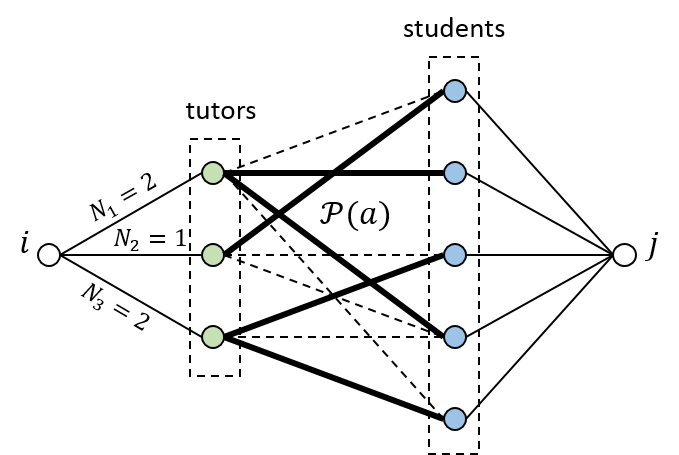
\includegraphics[scale=.65]{figs/maxflow.png}
\caption{Illustration of Max-Flow (MF) problem from $i$ to $j$ associated to the graph induced by the tutor-student pairs $\mathcal P(\alpha)$ with affinity not smaller than $a$. $E(\alpha)\subset \mathcal P(\alpha)$ is the set of edges having affinity exactly equal to $\alpha$. The edges from source $i$ to tutor $t$ has an annotated capacity $N_t$. All the other edges have unitary capacity. In this case, the optimal value is $|S'|=5$ hence each student is assigned to a tutor. The edges in bold constitute an optimal solution for MF($\alpha$).}
\label{fig:MF}
\end{figure}




\subsection{Min-Cost Flow (MCF)} \label{sec:mcf}

We now finally discuss how to solve line \ref{line:hard} of our main Algorithm \ref{alg:lexmax}.

We suppose we have already solved \eqref{eq:maxmin1} and found the maximum affinity $\widetilde{y}_k$ such that all students get one tutor each with affinity at least $y_k$. Now, we need to find the allocation $x^*$ with the minimum number of tutor-student pairs with affinity equal to $\widetilde{y}_k$. 

This problem can be reformulated via a Min-Cost flow problem (see \cite{bazaraa2011linear}, Ch. 9) or equivalently as a Transportation Problem (see \cite{bazaraa2011linear}, Ch. 10), since the tutor-student graph is bipartite. 

We remark that, as in the case of Max-Flow, there exist efficient \emph{polynomial} algorithms for solving such combinatorial problems \cite{bazaraa2011linear}.

In analogy to the previous section, let us describe the Min-Cost flow formulation. We first construct the same capacitated graph as in Section \ref{sec:MF}. Moreover, we append a cost to each edge, being equal to 1 if the corresponding tutor-student pair has affinity equal to $y_k$ (i.e., $E(y_k)$) and 0 otherwise. Then, the Min-Cost formulation simply asks to find the (maximum) flow of value $|S'|$ from $i$ to $j$ with minimum total cost (see Fig. \ref{fig:MCF}), while fulfilling the capacity constraints on the edges. In such a way, the number of tutor-student pairs with minimum affinity $y_k$ is minimized and the lexicographic maximization is sought.

\begin{figure}
\centering
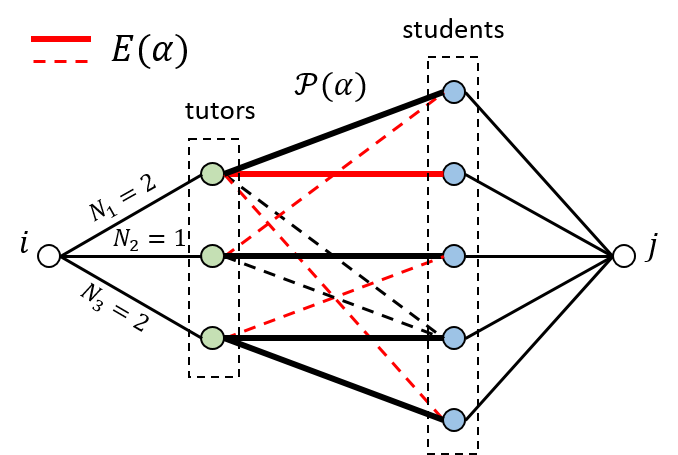
\includegraphics[scale=.65]{figs/mincost.png}
\caption{(continued from Fig. \ref{fig:MF}). Solving (MCF) allows to minimize the n. of pairs with affinity equal to $\alpha$ ($=1$ in this case, $=3$ in Fig. \ref{fig:MF}) while still assigning one tutor to each student. The edges in bald constitute the optimal tutor-student assignment; dashed edges denote all other tutor-student pairs; red edges are the ones with minimum affinity $y_k$, that one wants to avoid.}
\label{fig:MCF}
\end{figure}


\section{Large scale scenario} \label{sec:clustering}

Even though the complexity of the iterative max-min Algorithm \ref{alg:lexmax} is polynomial (hence, tractable) in the input size, we may need to resort to heuristics to simplify the problem in the case of large scale scenarios (large number of student $|S|$, tutors $|T|$ and affinity values $M$). 

One possibility is to split the problem into several smaller sub-problems that can then be solved in parallel.

 The idea is to partition the set of tutors $T$ into $n$ subsets $T_1,\dots,T_n$ and, similarly, the set of students $S$ into $S_1,\dots,S_n$ and solve $n$ max-min allocation problems in parallel over each ``cluster'' $(T_i,S_i)$. Clearly, this procedure is optimal only if the problem is fully decoupled over different clusters, i.e., the affinity between students and tutors belonging to different clusters is null. Hence, in order to get a good approximation of the original problem we should cluster the graph such that the inter-cluster affinity is low (see Fig. \ref{fig:clusters}). On the other hand, we should also ensure the clusters to have comparable size, in order to well balance the load among different processors.
This can be achieved, e.g., via the bipartite graph clustering technique in \cite{zha2001bipartite}.

Once having found an appropriate clustering, the iterative max-min Algorithm \ref{alg:lexmax} is ran in parallel over each (small) cluster $(T_i,S_i)$. Notice that this is equivalent to setting to zero all inter-cluster affinities $a_{s,t}$ with $s\in S_i,t\in T_j$ with $i\ne 0$. 

\begin{figure}
\centering
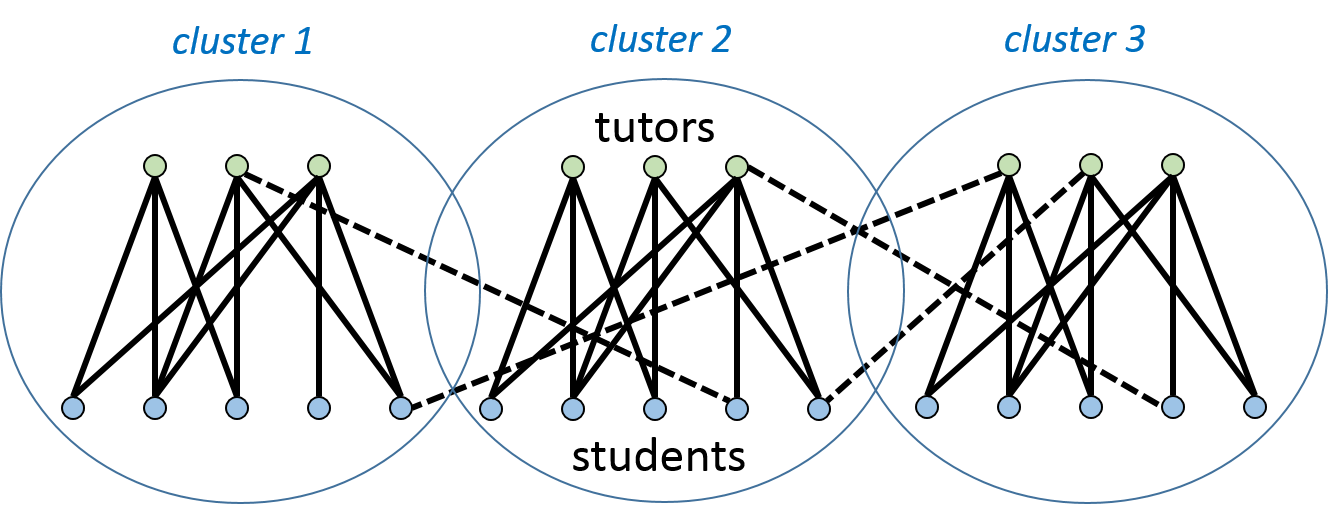
\includegraphics[scale=.5]{figs/clusters.png}
\caption{Tutor-student clustering. Iterative max-min Algorithm \ref{alg:lexmax} is run in parallel over different clusters. This is equivalent to setting to zero all inter-cluster affinity values, corresponding to dashed edges.}
\label{fig:clusters}
\end{figure}


\section{Online assignment}

As time goes by, some students may depart and/or new students may subscribe to the platform, so the tutor-student assignment must be modified in an online fashion in order to deal with the new situation.

We have fundamentally two ways to deal with this online scenario.
The optimal way is to recompute from scratch the overall new tutor-student assignment, by taking into account the new situation. 

However, recomputing a new allocation from scratch may be too time costly, as we may need to provide a decent choice to a student that logs in for the first time. For this reason, we suggest to exploit the clustering idea described in Section \ref{sec:clustering}. Each time a new student or tutor appears,

\begin{itemize}
\item we decide which cluster $(S_i,T_i)$ she will be attached to
\item we recompute the iterative max-min solution \emph{only} over the selected cluster
\end{itemize}

We finally remark that, when a new allocation is computed, the only student-tutor pair assignments that need to be maintained are those who currently have an ongoing conversation.




\bibliographystyle{plain}
\bibliography{bib_frateli}

\end{document}



